\documentclass[11pt,a4paper]{article}
\usepackage[utf8]{inputenc}
\usepackage[T1]{fontenc}
\usepackage[english]{babel}
\usepackage{geometry}
\geometry{margin=2.5cm}
\usepackage{hyperref}
\hypersetup{colorlinks=true, linkcolor=blue, urlcolor=blue}
\usepackage{listings}
\usepackage{xcolor}
\usepackage{enumitem}
\usepackage{titlesec}
\usepackage{natbib}
\bibliographystyle{plainnat}
\usepackage{tikz}
\usetikzlibrary{shapes, arrows.meta, positioning, fit, calc}

\lstset{
  language=Python,
  basicstyle=\ttfamily\small,
  keywordstyle=\color{blue},
  stringstyle=\color{red},
  commentstyle=\color{gray},
  breaklines=true,
  frame=single,
  numbers=left
}

\definecolor{gateblue}{HTML}{2563EB}
\definecolor{passgreen}{HTML}{16A34A}
\definecolor{failred}{HTML}{DC2626}
\definecolor{unverorange}{HTML}{EA580C}
\definecolor{mlopsindigo}{HTML}{4338CA}
\definecolor{proclight}{HTML}{E5E7EB}
\definecolor{notebookpurple}{HTML}{7C3AED}
\definecolor{phasedark}{HTML}{374151}

\tikzset{
  basenode/.style={draw, thick, minimum width=3.2cm, minimum height=0.8cm, align=center, font=\sffamily\small},
  notebook/.style={basenode, rounded corners=6pt, fill=notebookpurple, text=white, font=\sffamily\small\bfseries},
  gate/.style={basenode, rounded corners=3pt, fill=gateblue, text=white, font=\sffamily\small\bfseries},
  proc/.style={basenode, fill=proclight, text=phasedark},
  passnode/.style={basenode, rounded corners=6pt, fill=passgreen, text=white, font=\sffamily\small\bfseries},
  failnode/.style={basenode, rounded corners=6pt, fill=failred, text=white, font=\sffamily\small},
  unvernode/.style={basenode, rounded corners=6pt, fill=unverorange, text=white, font=\sffamily\small},
  mlopsnode/.style={basenode, rounded corners=6pt, fill=mlopsindigo, text=white, font=\sffamily\small\bfseries},
  arr/.style={-{Stealth[length=5pt]}, thick, black},
  fbarrow/.style={-{Stealth[length=5pt]}, thick, failred, dashed},
  uvarrow/.style={-{Stealth[length=5pt]}, thick, unverorange, dashed},
  phasebar/.style={dashed, thick, phasedark},
  phasetxt/.style={font=\sffamily\tiny, text=phasedark, rotate=90, anchor=south}
}

\title{Methodological Audit of Machine Learning Notebooks}
\author{Audit Engine AI}
\date{}

\begin{document}
\maketitle

\section{Context}

To audit the methodology of Machine Learning before MLOps, there is no turnkey commercial agent, but rather a deterministic normative workflow based on scientific rigor and bias prevention.

\section{ML Methodological Audit Normative}

The AI engine must evaluate the code by searching for anti-methodological patterns divided into three main axes:

\subsection{Data Leakage --- Critical Severity}

\begin{itemize}
  \item \textbf{Disordered Fit/Transform:} \texttt{StandardScaler}, \texttt{MinMaxScaler}, or other transformers apply \texttt{.fit()} or \texttt{.fit\_transform()} to the entire dataset before executing \texttt{train\_test\_split}.
  \item \textbf{Target Leakage:} Feature creation computing global statistical aggregations that involve the target variable (\texttt{y}).
  \item \textbf{Viciated Cross-Validation:} Application of dimensionality reduction (e.g., PCA) or global scaling before cross-validation, instead of inside a scikit-learn Pipeline.
\end{itemize}

\subsection{Reproducibility and Data Splitting}

\begin{itemize}
  \item \textbf{Randomness Control:} Absence of global or local seeds (\texttt{random\_state}, \texttt{seed}) in data splits, clustering algorithms, or stochastic models.
  \item \textbf{Wrong Split Strategy:} Use of standard random splitting (\texttt{random\_split}) on sequential or temporal data (requires Time-Series Split) or on severely imbalanced datasets (requires stratified splitting with \texttt{stratify}).
\end{itemize}

\subsection{Modeling and Metrics Coherence}

\begin{itemize}
  \item \textbf{Inadequate Metric:} Evaluation based on Accuracy for imbalanced class problems instead of F1-Score, PR-AUC, or ROC-AUC.
  \item \textbf{Missing Baseline:} Training the final model without prior comparison against a naive or reference model (dummy/baseline classifier).
\end{itemize}

\section{Orchestration Flow for the Audit Engine AI}

\subsection{Context Extraction and AST (Static Syntax)}

Before passing the code to the LLM, a script extracts the Data Flow Graph from the AST of the normalized code. This locates which cells declare dataframes, transformations, and where the first \texttt{.fit()} occurs.

\subsection{Specialized Sub-Agent Evaluation}

\begin{itemize}
  \item \textbf{Leakage and Transformations Agent:} Analyzes solely the temporal sequence of data flow between DataFrames to detect Data Leakage.
  \item \textbf{Metrics and Validation Agent:} Analyzes the model arguments and metrics called in the evaluation subset.
\end{itemize}

\subsection{Structured Consolidation}

The engine combines failures and generates a deterministic JSON response to automate corrections.

\section{Recommended Agent Output Schema}

\begin{lstlisting}
{
  "cell_index": 5,
  "severity": "CRITICAL",
  "category": "Data Leakage",
  "issue": "StandardScaler.fit_transform() executed
            before train_test_split()",
  "line_code": "X_scaled = scaler.fit_transform(X)",
  "suggested_fix": "X_train, X_test = train_test_split(X, ...)\n
                    X_train_scaled = scaler.fit_transform(X_train)\n
                    X_test_scaled = scaler.transform(X_test)"
}
\end{lstlisting}

\clearpage

\section{Audit Workflow Diagram}

\begin{figure}[ht]
\centering
\resizebox{\textwidth}{!}{%
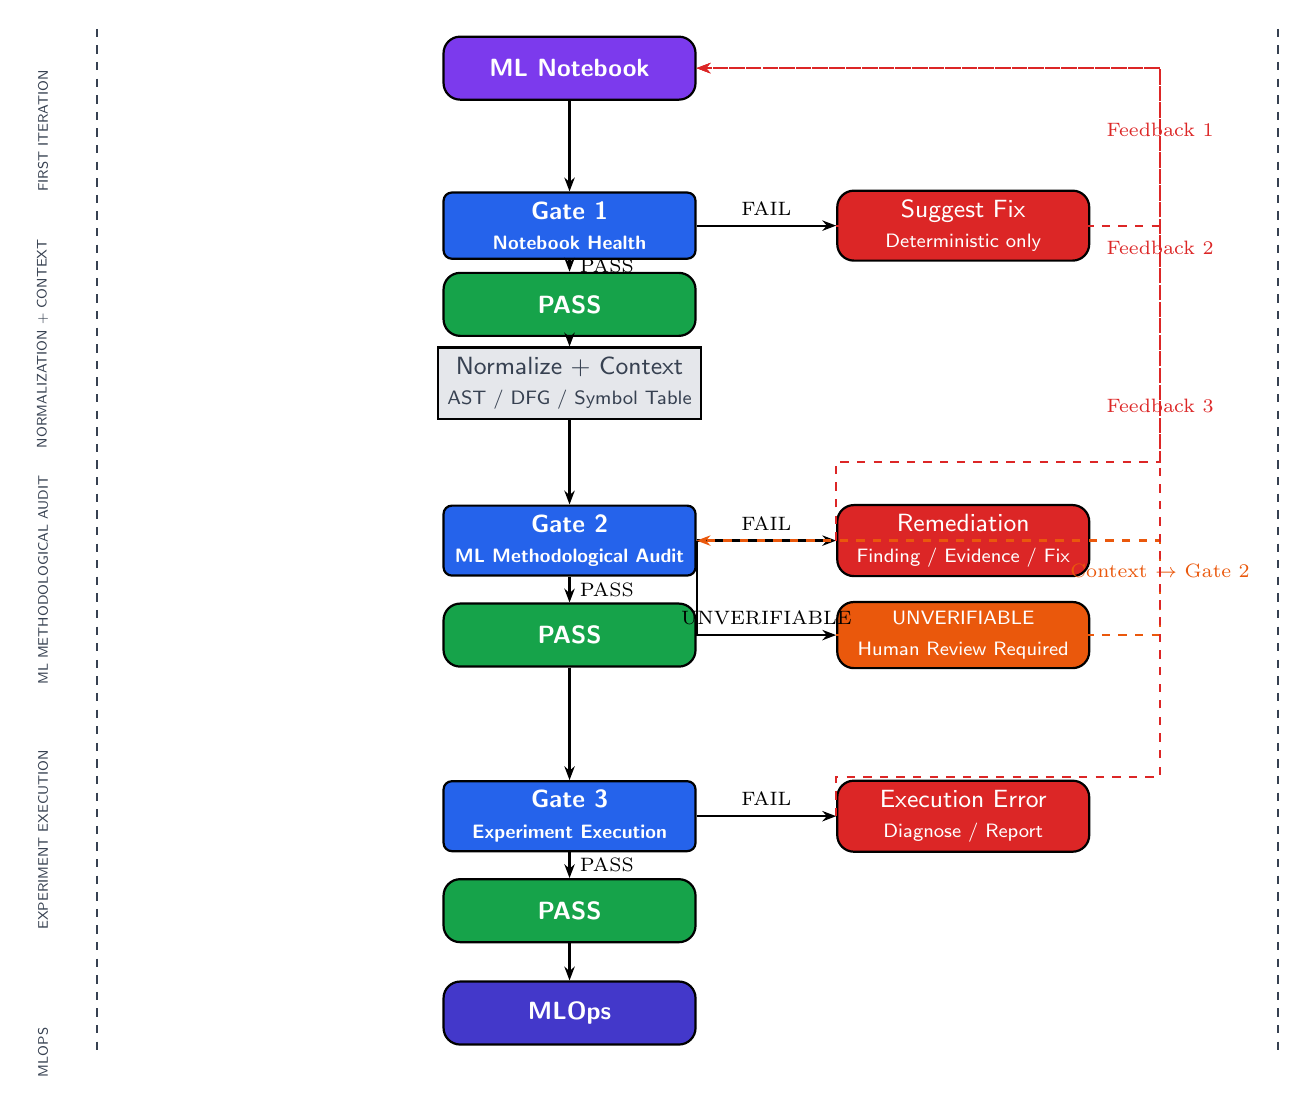
\begin{tikzpicture}

% ===== MAIN SPINE =====
\node[notebook]  (NB) at (8, 0)    {ML Notebook};
\node[gate]      (G1) at (8, -2)   {Gate 1\\{\scriptsize Notebook Health}};
\node[proc]      (NRM) at (8, -4)  {Normalize + Context\\{\scriptsize AST / DFG / Symbol Table}};
\node[gate]      (G2) at (8, -6)   {Gate 2\\{\scriptsize ML Methodological Audit}};
\node[gate]      (G3) at (8, -9.5) {Gate 3\\{\scriptsize Experiment Execution}};
\node[mlopsnode] (OPS) at (8, -12) {MLOps};

% ===== GATE 1 BRANCH =====
\node[passnode]   (P1) at (8, -3)   {PASS};
\node[failnode]   (F1) at (13, -2)  {Suggest Fix\\{\scriptsize Deterministic only}};

% ===== GATE 2 BRANCH =====
\node[passnode]   (P2) at (8, -7.2) {PASS};
\node[failnode]   (F2) at (13, -6)  {Remediation\\{\scriptsize Finding / Evidence / Fix}};
\node[unvernode]  (U2) at (13, -7.2){{\scriptsize UNVERIFIABLE}\\{\scriptsize Human Review Required}};

% ===== GATE 3 BRANCH =====
\node[passnode]   (P3) at (8, -10.7){PASS};
\node[failnode]   (F3) at (13, -9.5){Execution Error\\{\scriptsize Diagnose / Report}};

% ===== MAIN FLOW ARROWS =====
\draw[arr] (NB)  -- (G1);
\draw[arr] (G1)  -- node[right,font=\scriptsize] {PASS} (P1);
\draw[arr] (P1)  -- (NRM);
\draw[arr] (NRM) -- (G2);
\draw[arr] (G2)  -- node[right,font=\scriptsize] {PASS} (P2);
\draw[arr] (P2)  -- (G3);
\draw[arr] (G3)  -- node[right,font=\scriptsize] {PASS} (P3);
\draw[arr] (P3)  -- (OPS);

% ===== FAIL BRANCHES =====
\draw[arr] (G1.east) -- node[above,font=\scriptsize] {FAIL} (F1);
\draw[arr] (G2.east) -- node[above,font=\scriptsize] {FAIL} (F2);
\draw[arr] (G2.east) |- node[near end,above,font=\scriptsize] {UNVERIFIABLE} (U2);
\draw[arr] (G3.east) -- node[above,font=\scriptsize] {FAIL} (F3);

% ===== FEEDBACK LOOPS =====
\draw[fbarrow] (F1.west) |- (15.5, -2) |- (NB.east)
  node[pos=0.25,above,font=\scriptsize] {\textcolor{failred}{Feedback 1}};
\draw[fbarrow] (F2.west) |- (15.5, -5) |- (NB.east)
  node[pos=0.25,above,font=\scriptsize] {\textcolor{failred}{Feedback 2}};
\draw[uvarrow] (U2.west) |- (15.5, -7.2) |- (G2.east)
  node[pos=0.25,above,font=\scriptsize] {\textcolor{unverorange}{Context $\rightarrow$ Gate 2}};
\draw[fbarrow] (F3.west) |- (15.5, -9) |- (NB.east)
  node[pos=0.25,above,font=\scriptsize] {\textcolor{failred}{Feedback 3}};

% ===== LEFT PHASE BARS =====
\draw[phasebar] (2, 0.5) -- (2, -12.5);
\node[phasetxt] at (1.5, -0.8)   {FIRST ITERATION};
\node[phasetxt] at (1.5, -3.5)   {NORMALIZATION + CONTEXT};
\node[phasetxt] at (1.5, -6.5)   {ML METHODOLOGICAL AUDIT};
\node[phasetxt] at (1.5, -9.8)   {EXPERIMENT EXECUTION};
\node[phasetxt] at (1.5, -12.5)  {MLOPS};

% ===== RIGHT DECORATIVE BAR =====
\draw[phasebar] (17, 0.5) -- (17, -12.5);

\end{tikzpicture}%
}
\caption{Audit Workflow --- Three-gate deterministic methodology for ML notebook validation prior to MLOps execution.}
\label{fig:audit-flow}
\end{figure}

\section*{References}

\begingroup
\renewcommand{\section}[2]{}
\begin{thebibliography}{99}

\bibitem[Yang et~al.(2022)]{yang2022leakage}
Yang, C., Brower-Sinning, R., Lewis, G., and K\"{a}stner, C.
\newblock Data leakage in notebooks: Static detection and better processes.
\newblock In \emph{Proc.\ 37th IEEE/ACM Int.\ Conf.\ on Automated Software Engineering (ASE~'22)}, 2022.
\newblock \url{https://doi.org/10.1145/3551349.3556918}

\bibitem[Subotić et~al.(2022)]{subotic2022static}
Subotić, P., Bojanić, U., and Stojić, M.
\newblock Statically detecting data leakages in data science code.
\newblock In \emph{Proc.\ 11th ACM SIGPLAN Int.\ Workshop on the State Of the Art in Program Analysis (SOAP~'22)}, 2022.
\newblock \url{https://doi.org/10.1145/3520313.3534657}

\bibitem[Kaufman et~al.(2012)]{kaufman2012leakage}
Kaufman, S., Rosset, S., Perlich, C., and Stitelman, O.
\newblock Leakage in data mining: Formulation, detection, and avoidance.
\newblock \emph{ACM Trans.\ on Knowledge Discovery from Data}, 6(4):15:1--15:21, 2012.
\newblock \url{https://doi.org/10.1145/2382577.2382579}

\bibitem[Breck et~al.(2017)]{breck2017mltest}
Breck, E., Cai, S., Nielsen, E., Salib, M., and Sculley, D.
\newblock The ML test score: A rubric for ML production readiness and technical debt reduction.
\newblock In \emph{Proc.\ 2017 IEEE Int.\ Conf.\ on Big Data (Big Data~'2017)}, pages 1123--1132, 2017.
\newblock \url{https://doi.org/10.1109/BigData.2017.8258038}

\bibitem[Sculley et~al.(2015)]{sculley2015hidden}
Sculley, D., Holt, G., Golovin, D., Davydov, E., Phillips, T., Ebner, D., Chaudhary, V., Young, M., Crespo, J.-F., and Dennison, D.
\newblock Hidden technical debt in machine learning systems.
\newblock In \emph{Advances in Neural Information Processing Systems 28 (NIPS~2015)}, pages 2503--2511, 2015.
\newblock \url{https://papers.nips.cc/paper/5656-hidden-technical-debt-in-machine-learning-systems}

\bibitem[NIST(2023)]{nist2023airmf}
National Institute of Standards and Technology.
\newblock \emph{Artificial Intelligence Risk Management Framework (AI RMF 1.0)}, January 2023.
\newblock NIST AI 100-1.
\newblock \url{https://doi.org/10.6028/NIST.AI.100-1}

\end{thebibliography}
\endgroup

\end{document}
